\clearpage

{\color{red} This might become Section 4 (after the Methodology and before the result of the analysis on the Run 1+2 dataset). }

\section{Sensitivity studies}

In this section several sensitivity plots are presented, including 1D marginalized $\Delta\chi^{2}$ distributions and 2D confidence regions.

A 1D marginalized $\Delta\chi^{2}$ distribution is a plot of $\Delta\chi^{2}$ as a function of a single oscillation parameter. For each value 
of the parameter concerned, the other three oscillation parameters and the systematic parameters are marginalised by being allowed to float in 
the fit until $\chi^{2}$ (from equation \ref{eq:chisqtot}) is minimised; then the value of $\Delta\chi^{2}$ to be entered onto the plot is 
calculated as that value of $\chi^{2}$ minus the global minimum value. Each plot is made by fitting a single toy MC dataset, with statistical 
fluctuations not being included since it is clearer to view a single distribution. When they are not the parameter concerned, the input values 
to the toy datasets are shown in table \ref{tab:inputvalues}. 
\begin{table}[h]
\centering
\begin{tabular}{|c|c|}
\hline
 Parameter & Input value \\
  & when marginalised \\
\hline \hline
$\sin^{2}\theta_{23}$ & 0.56 \\
$\sin^{2}\theta_{13}$ & 0.024 \\
$\Delta m_{32}^{2}$ & 2.4$\times$10$^{-3}$ eV$^{2}$/c$^{4}$\\
$\delta_{CP}$ & 0 \\
\hline
\end{tabular}
\caption{Input values of the oscillation parameters to the toy MC datasets for the 1D marginalized $\Delta\chi^{2}$ distributions when they are not 
         the parameter concerned, i.e.\ when they are marginalised.}
\label{tab:inputvalues}
\end{table}

These distributions allow several checks to be made. First, the position of the minimum of $\Delta\chi^{2}$ can be checked against the true 
input value of the oscillation parameter. Second, a check can be made that only one minimum exists (except for $\sin^{2}\theta_{23}$, for 
which two minima are expected). Finally, they can be checked for any spikes or other unusual features. 

The 1D marginalized distributions for $\sin^{2}\theta_{23}$, $\sin^{2}\theta_{13}$, $\Delta m_{32}^{2}$ and $\delta_{CP}$ are shown in figures 
\ref{fig:1Dchisqtheta23}, \ref{fig:1Dchisqtheta13}, \ref{fig:1Dchisqdm23sq} and \ref{fig:1Dchisqdeltacp} respectively. Each of these figures shows 
the distributions from toy experiments with several different input values of the oscillation parameter concerned, and for both the Run 1+2 POT 
(1.43$\times$10$^{20}$) and the estimated final POT (7$\times$10$^{21}$). In all cases except $\delta_{CP}$, the fitter correctly recovers 
the input value of the oscillation parameter concerned.
 
In figure \ref{fig:1Dchisqtheta23}, the distributions show that the two minima of the distributions for $\sin^{2}\theta_{23}$ become less pronounced
as the true input values approach the centre of symmetry. Comparing the left and right plots, the two minima are more pronounced with more POT. Both of 
these features are expected. For $\sin^{2}\theta_{13}$, the $\Delta\chi^{2}$ distributions in figure \ref{fig:1Dchisqtheta13} are narrower at lower true 
input values, and also narrower with more POT. Meanwhile the distributions for $\Delta m_{32}^{2}$ are unaffected by the true input value, but are also 
narrower with more POT (see figure \ref{fig:1Dchisqdm23sq}).

The distributions for $\delta_{CP}$ are more difficult to interpret. They do show minima near the true input values, but it cannot be considered that 
these minima are recovering the true input values since $\Delta\chi^{2}$ is tiny and of the order of 10$^{-5}$. Although the distributions are narrower 
for more POT, they are still not convincing as $\Delta\chi^{2}$ is still very small. For this reason, a further study of the fitting of $\delta_{CP}$ 
was made, and the results are given in Appendix \ref{subsec:deltaCP}.

\begin{figure}[htbp]
\begin{center}
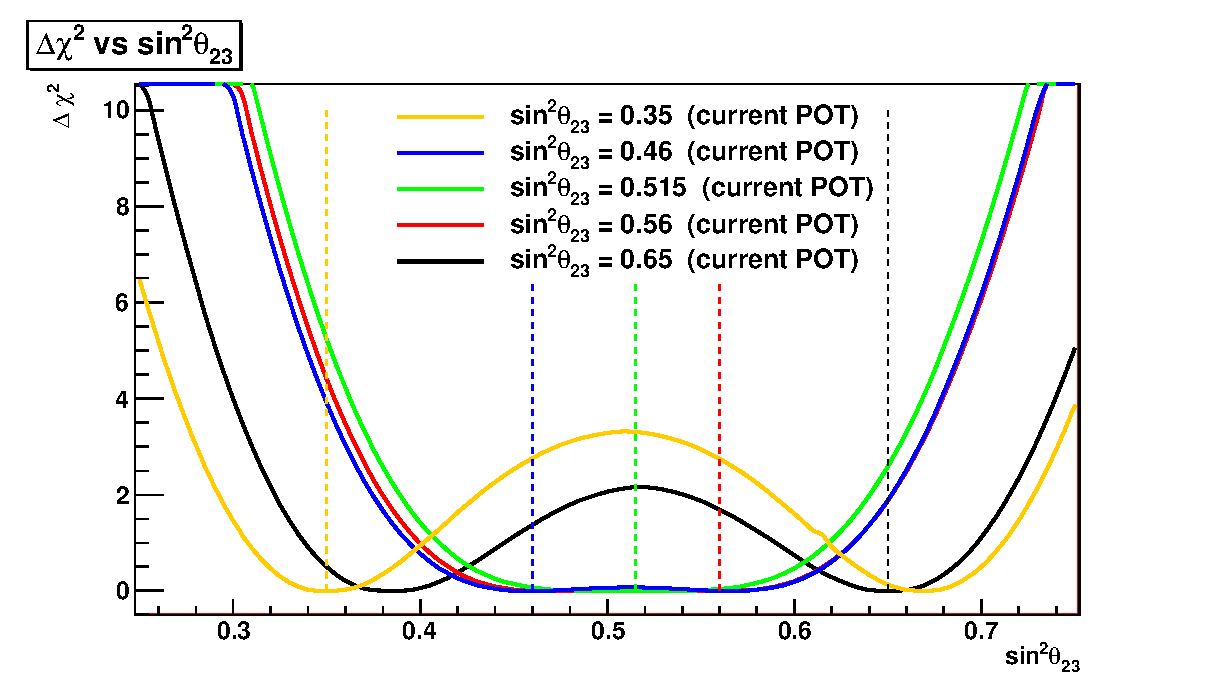
\includegraphics[width=0.5\textwidth]{images/validation/DeltaChisqVsTheta23CurrentSets.eps}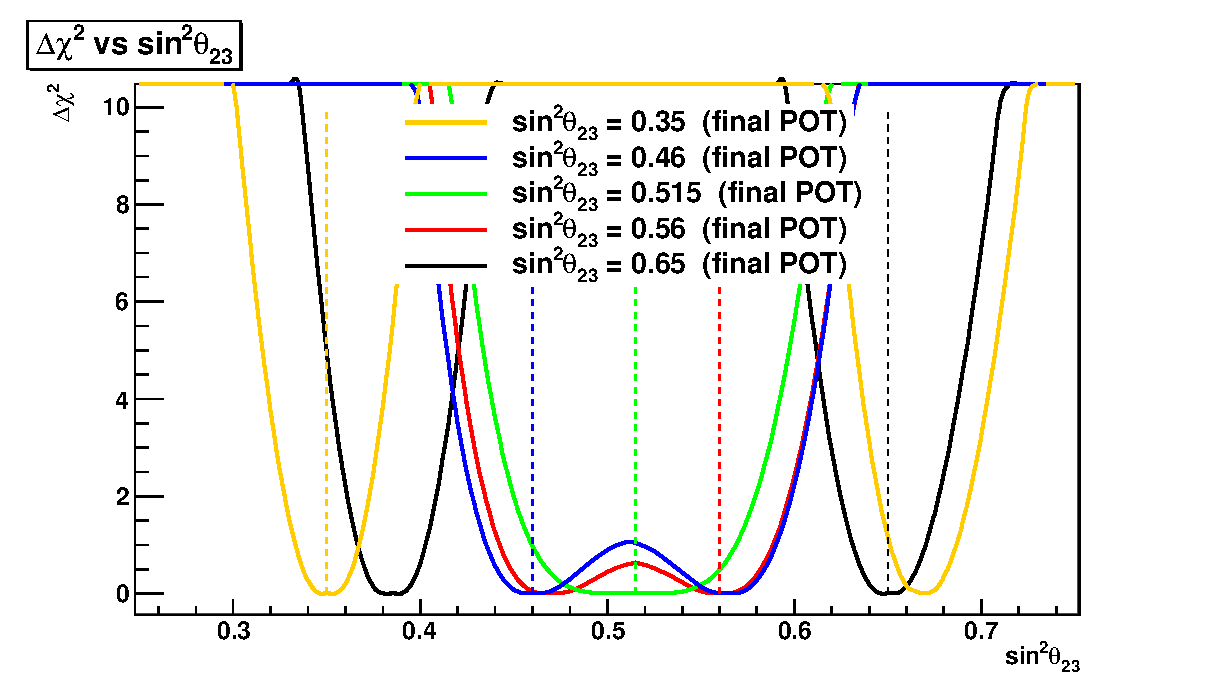
\includegraphics[width=0.5\textwidth]{images/validation/DeltaChisqVsTheta23Mock100Sets.eps}
\caption{1D marginalized $\Delta\chi^{2}$ distribution as a function of $\sin^{2}\theta_{23}$ for different true input values for the Run 1+2 POT (1.43$\times$10$^{20}$, left) 
and estimated final POT (7$\times$10$^{21}$, right)}
\label{fig:1Dchisqtheta23}
\end{center}
\end{figure}

\begin{figure}[htbp]
\begin{center}
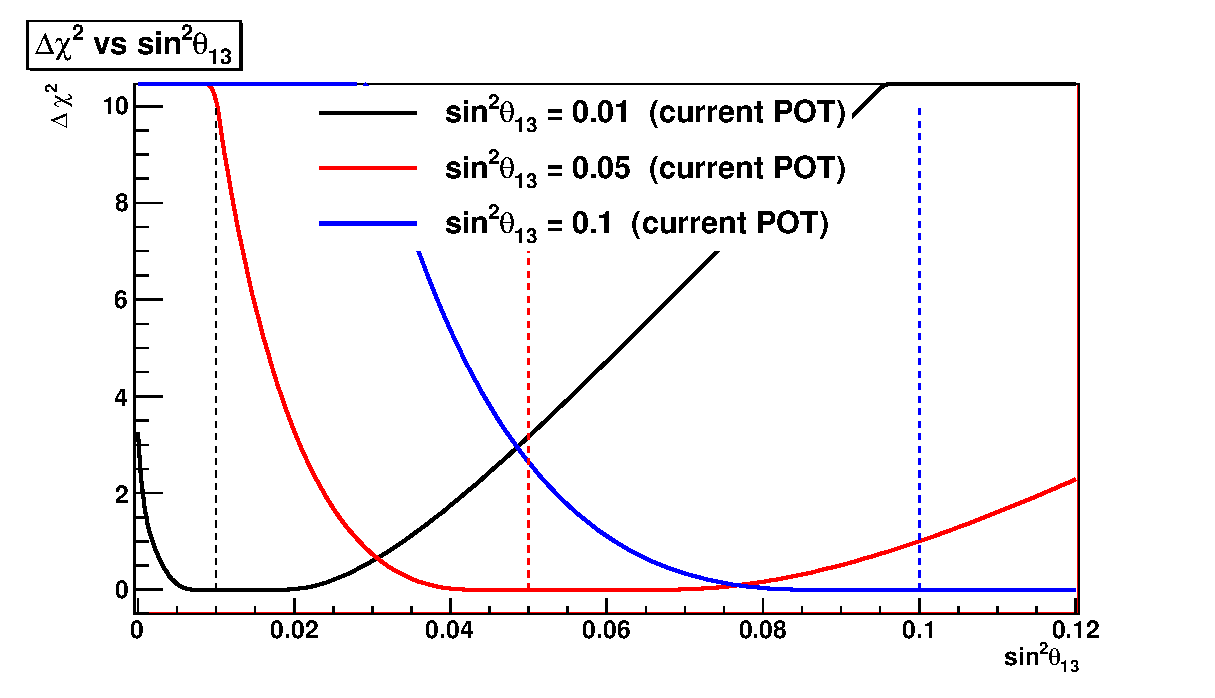
\includegraphics[width=0.5\textwidth]{images/validation/DeltaChisqVsTheta13CurrentSets.eps}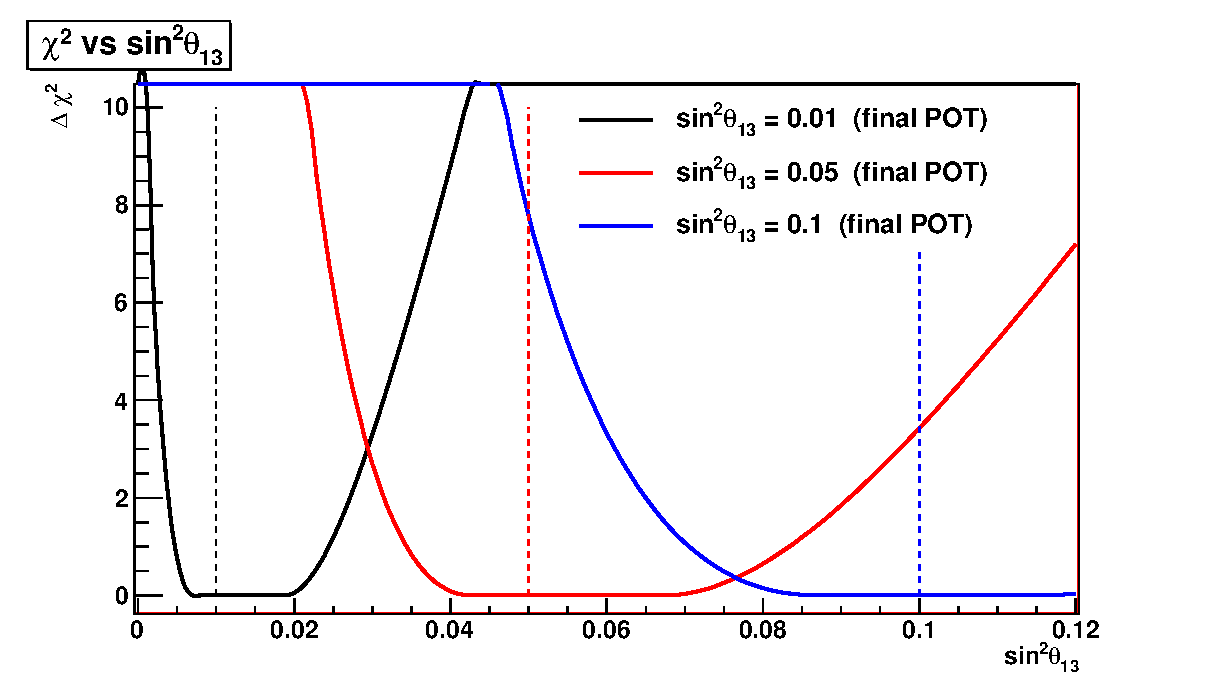
\includegraphics[width=0.5\textwidth]{images/validation/DeltaChisqVsTheta13Mock100Sets.eps}
\caption{ 1D marginalized $\Delta\chi^{2}$ distribution as a function of $\sin^{2}\theta_{13}$ for different true input values for the Run 1+2 POT (1.43$\times$10$^{20}$, left) 
and estimated final POT (7$\times$10$^{21}$, right).}
\label{fig:1Dchisqtheta13}
\end{center}
\end{figure}

\begin{figure}[htbp]
\begin{center}
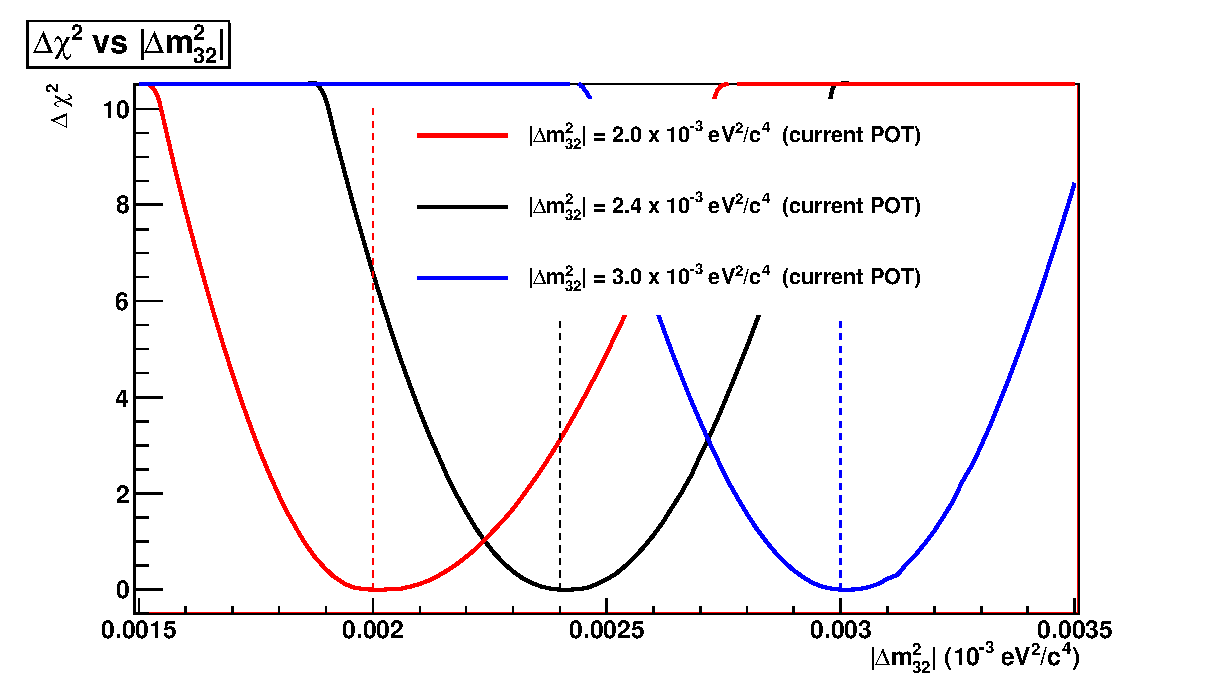
\includegraphics[width=0.5\textwidth]{images/validation/DeltaChisqVsDm23sqCurrentSets.eps}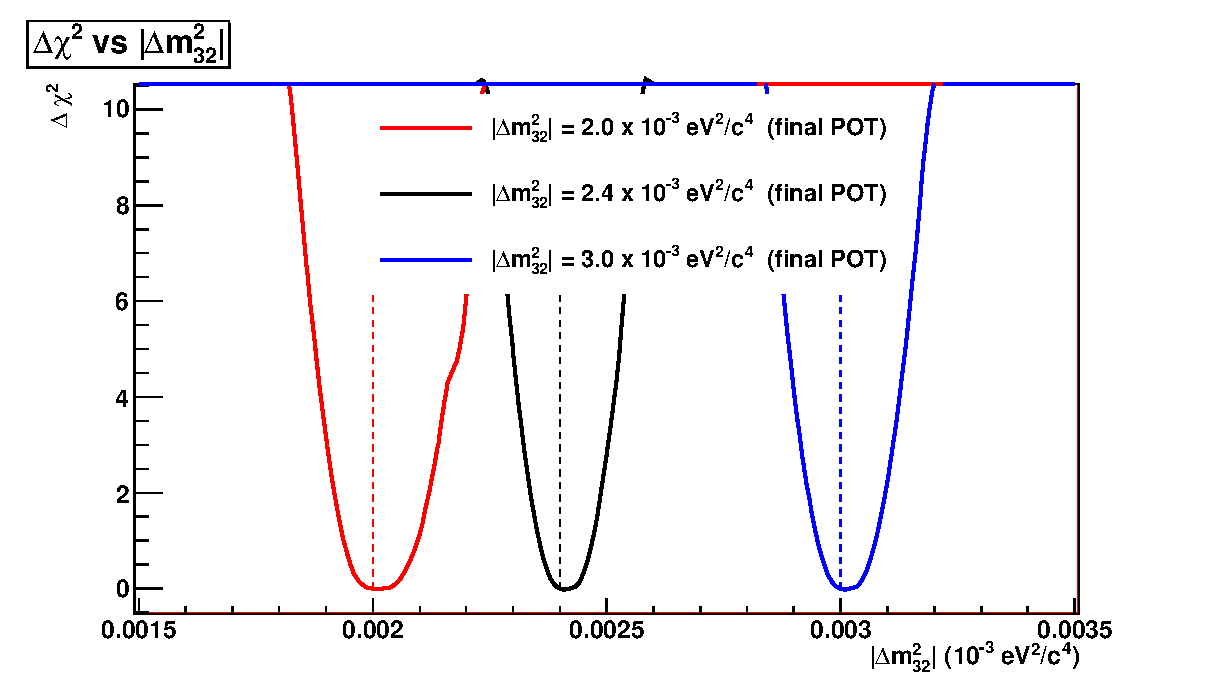
\includegraphics[width=0.5\textwidth]{images/validation/DeltaChisqVsDm23sq100Sets.eps}
\caption{ 1D marginalized $\Delta\chi^{2}$ distribution as a function of $\Delta m_{32}^{2}$ for different true input values for the Run 1+2 POT (1.43$\times$10$^{20}$, left) 
and estimated final POT (7$\times$10$^{21}$, right)}
\label{fig:1Dchisqdm23sq}
\end{center}
\end{figure}

\begin{figure}[htbp]
\begin{center}
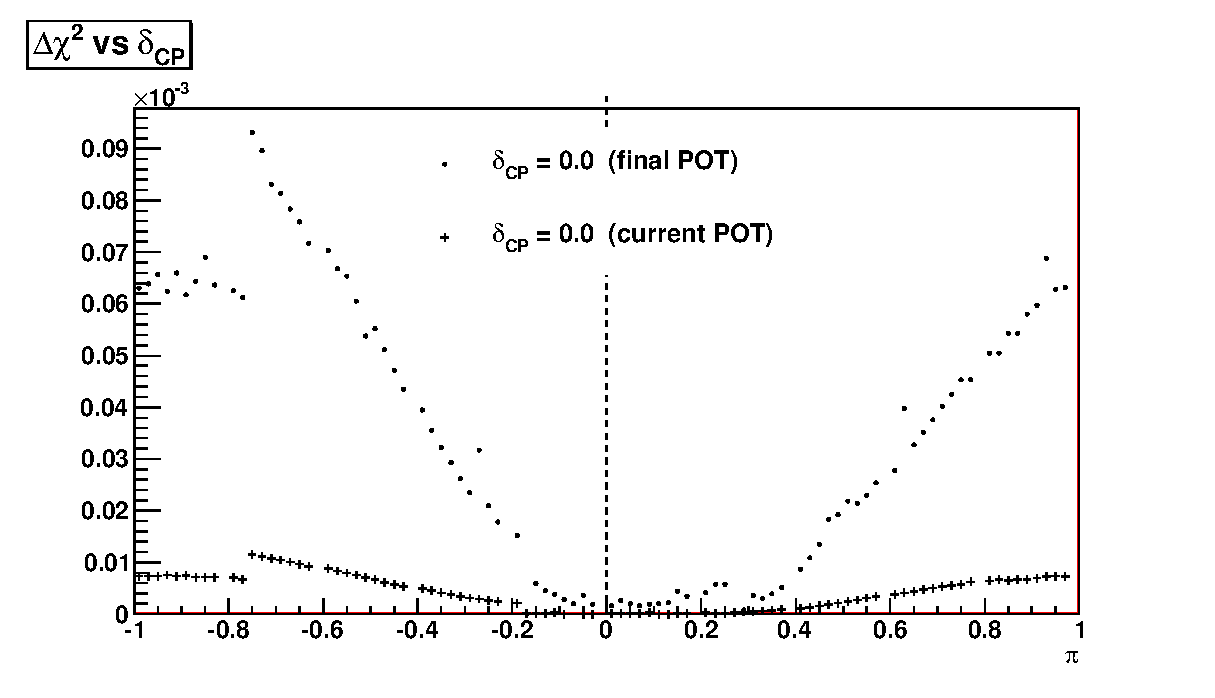
\includegraphics[width=0.5\textwidth]{images/validation/DeltaChisqVsDeltaCPSet0.eps}
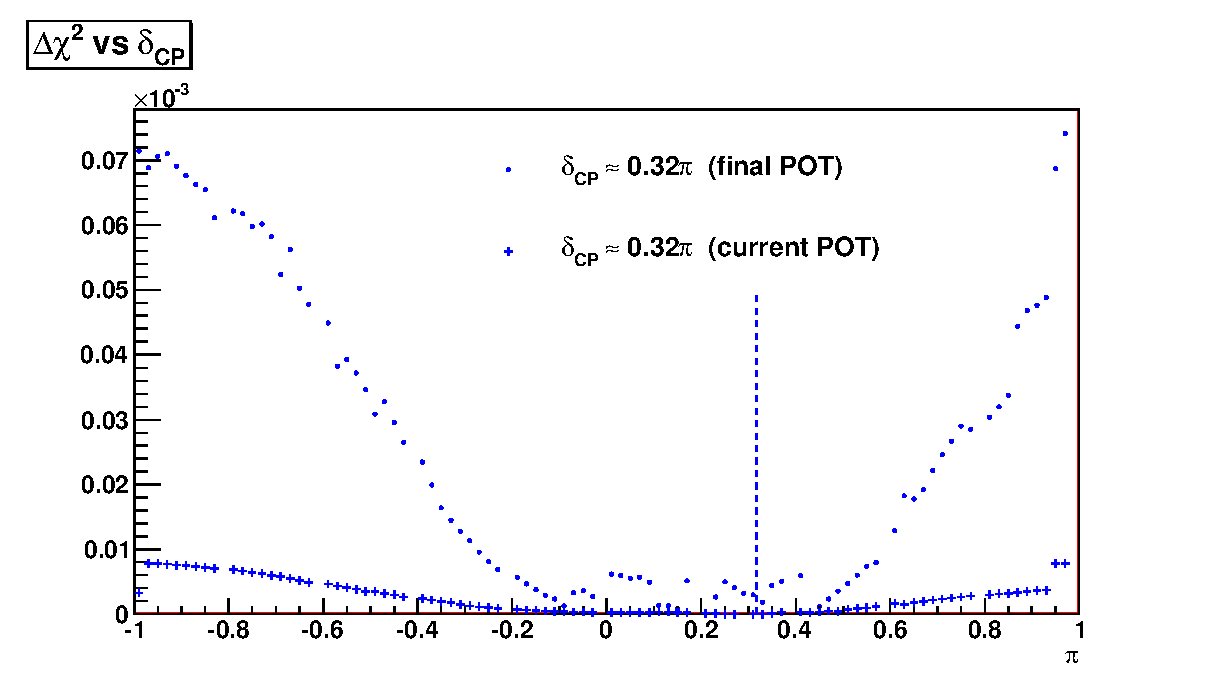
\includegraphics[width=0.5\textwidth]{images/validation/DeltaChisqVsDeltaCPSet1.eps}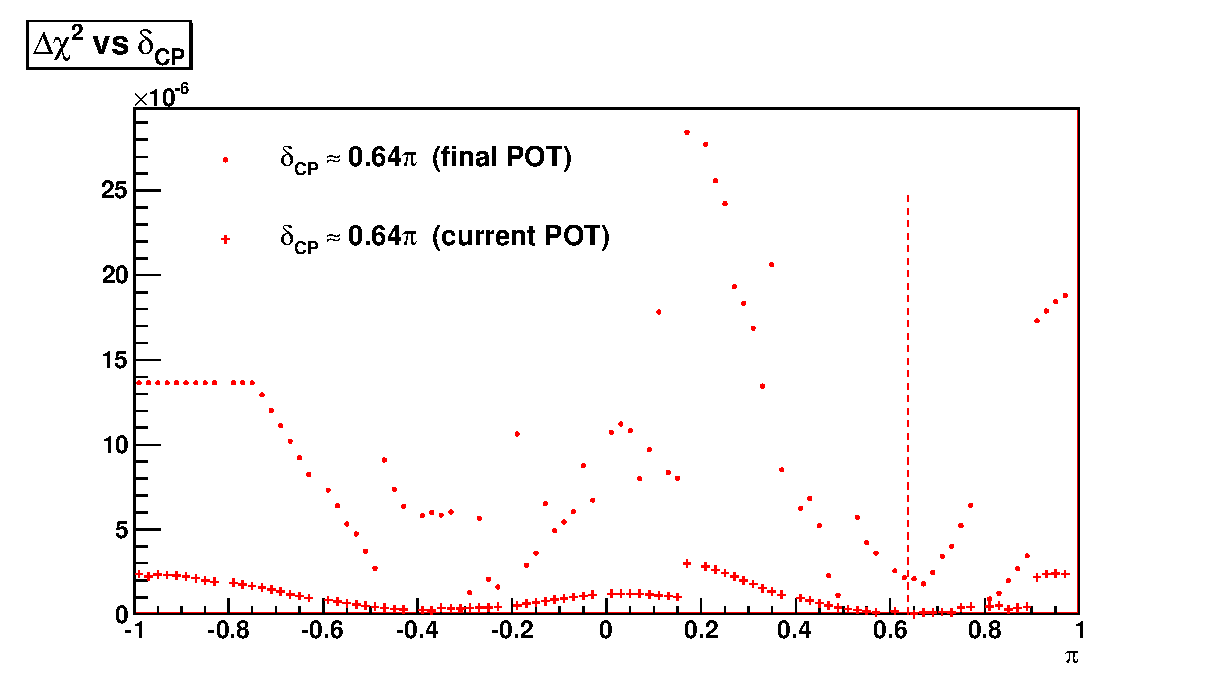
\includegraphics[width=0.5\textwidth]{images/validation/DeltaChisqVsDeltaCPSet2.eps}
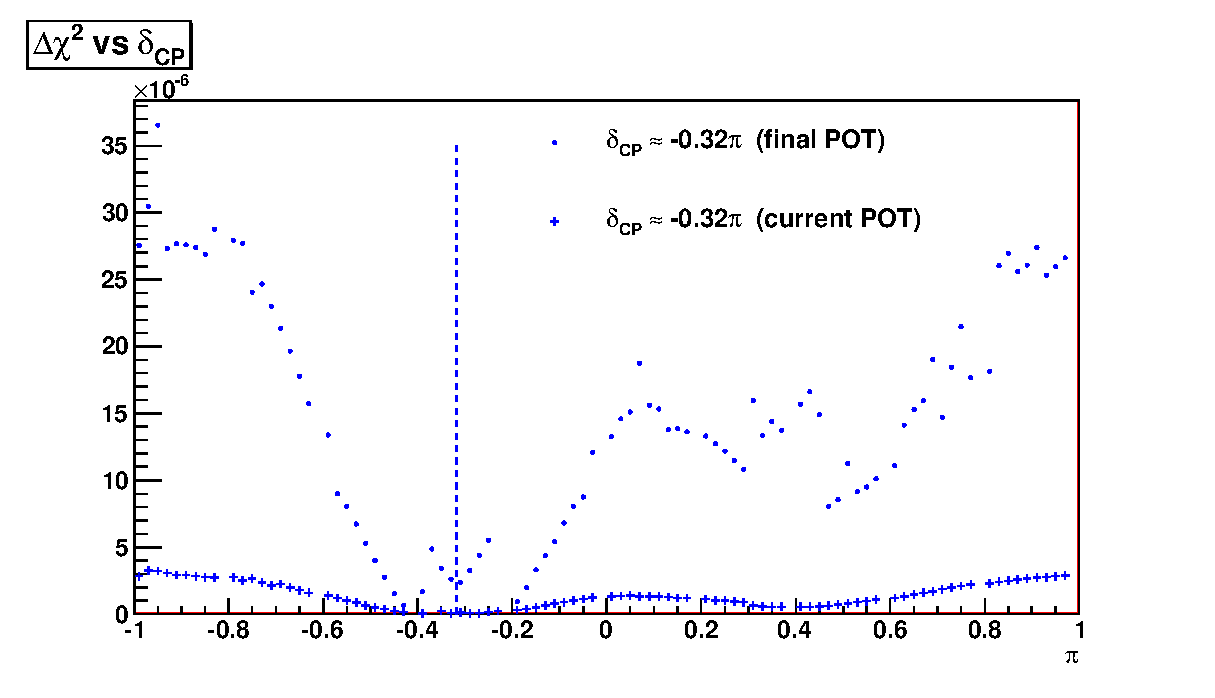
\includegraphics[width=0.5\textwidth]{images/validation/DeltaChisqVsDeltaCPSet3.eps}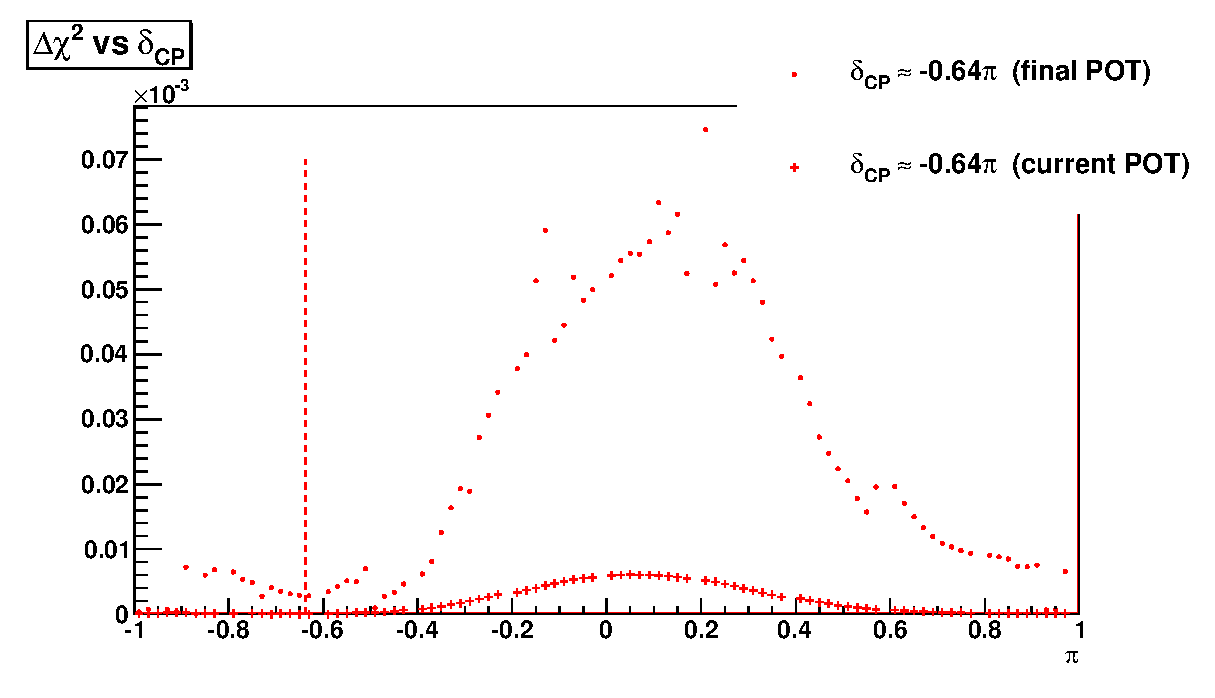
\includegraphics[width=0.5\textwidth]{images/validation/DeltaChisqVsDeltaCPSet4.eps}
\caption{ 1D marginalized $\Delta\chi^{2}$ distribution as a function of $\delta_{CP}$ for different true input values at Run 1+2 POT (1.43$\times$10$^{20}$) and estimated final POT 
(7$\times$10$^{21}$).}
\label{fig:1Dchisqdeltacp}
\end{center}
\end{figure}

{\color{red}{TO INCLUDE: Comparison of 1D $\Delta\chi^{2}$ for joint vs standalone. Worked on this today but need to check }}

\ \ \\


A 2D confidence region is made by producing a 2D plot of $\Delta\chi^{2}$ as a function of two oscillation parameters in a rectangular grid, with
the other two oscillation parameters and the systematic parameters being marginalised. The bin widths and ranges of these grids are shown in 
table \ref{tab:binning}, and there is a grid point at the centre of each rectangle. Using the $\Delta\chi^{2}$ plot, the confidence region is 
drawn in such a way that it includes all parts of the 2D oscillation parameter space for which $\Delta\chi^{2}$ $<$ 2.30 (68\% confidence) or 
4.61 (90\% confidence). For each 2D confidence region, the fitted values of the two marginalised oscillation parameters are also shown by 
superimposing them on the confidence contours.

All 2D confidence regions shown in this section are for the estimated final POT (7$\times$10$^{21}$). However the 2010 version of the systematic 
parameters was used, and the confidence regions should become slightly smaller with impoved analysis of those parameters. 

\begin{table}[h]
\centering
\begin{tabular}{|c|c|c|c|c|}
\hline
 Parameter & Minimum & Maximum & Step & \# bins\\
\hline \hline
$\sin^{2}2\theta_{23}$ & 0.9 & 1.0 & 0.002 & 50\\
$\sin^{2}2\theta_{13}$ & 0.0 & 0.264 & 0.008 & 33 \\
$\Delta m_{32}^{2} (\times 10^{-3} eV^{2}/c^{4})$ & 2.0& 3.0& 0.05 & 50 \\
$\delta_{CP}$ & -$\pi$ & $\pi$& $\frac{2\pi}{50}$ & 50\\
\hline
\end{tabular}
\caption{Summary of the binning used for the 2D confidence contours}
\label{tab:binning}
\end{table}

The 68\% and 90\% confidence regions obtained by the joint oscillation analysis are shown in the $\sin^{2}2\theta_{13}$-$\delta_{CP}$ parameter space 
in figure \ref{fig:jointapp}, in which $\sin^{2}2\theta_{23}$, $\Delta m_{32}^{2}$ and the systematic parameters are marginalised. The fitted values 
of $\sin^{2}2\theta_{23}$ and $\Delta m_{32}^{2}$ are shown at each point in the $\sin^{2}2\theta_{13}$-$\delta_{CP}$ space in figure \ref{fig:jointappfitted}. 
Statistical fluctuations were not applied to the toy dataset as this would have meant that there were different input values at different grid points. 
Confidence regions are also shown in the $\sin^{2}2\theta_{23}$-$\Delta m_{32}^{2}$ parameter space in figure \ref{fig:jointdisapp}, and the fitted 
values of $\sin^{2}2\theta_{13}$ and $\delta_{CP}$ in that space are presented in figure \ref{fig:jointdisappfitted}. 

\begin{figure}[htbp]
\begin{center}
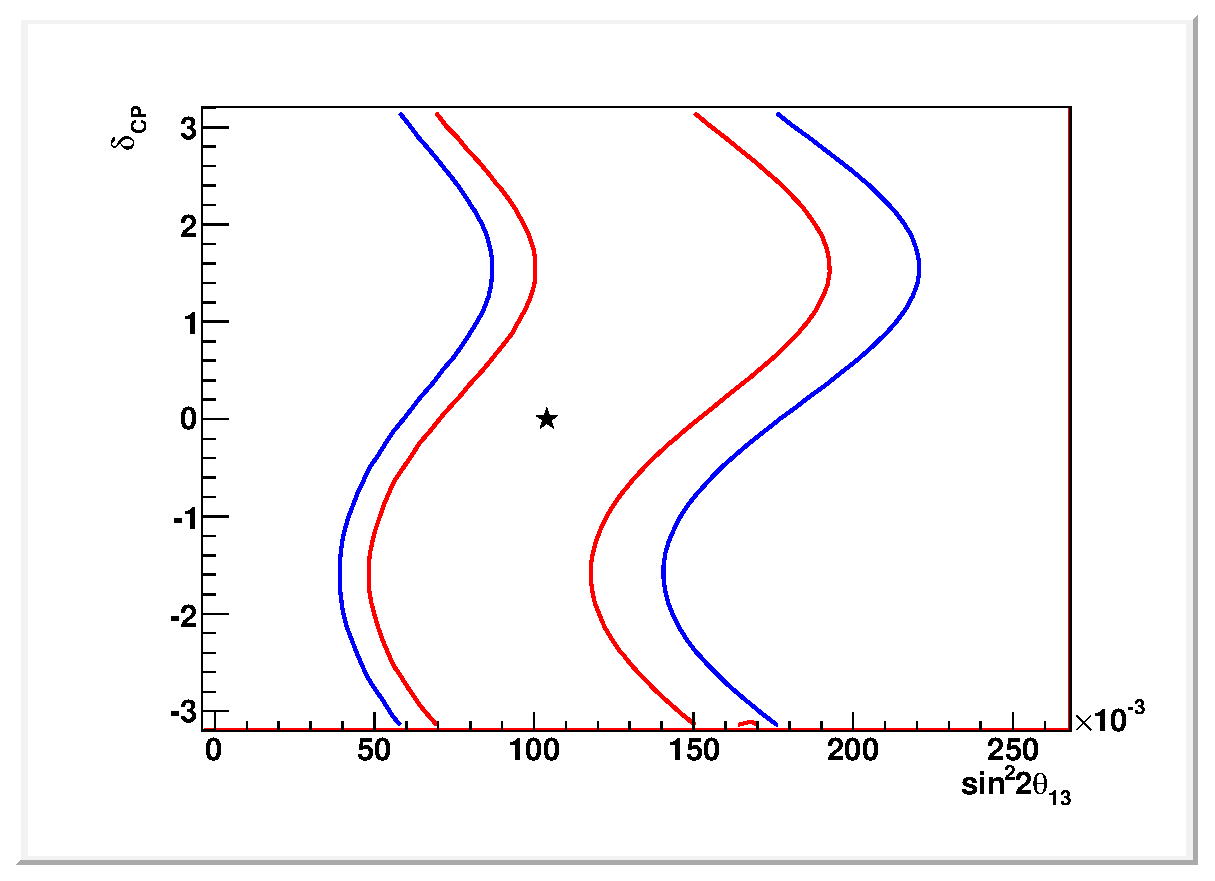
\includegraphics[width=0.7\textwidth]{images/validation/AppContoursJointOAMock100New.eps}
\caption{2D confidence regions for the joint oscillation analysis in the $\sin^{2}2\theta_{13}$-$\delta_{CP}$ parameter space for the estimated final POT (7$\times$10$^{21}$).}
\label{fig:jointapp}
\end{center}
\end{figure}


\begin{figure}[htbp]
\begin{center}
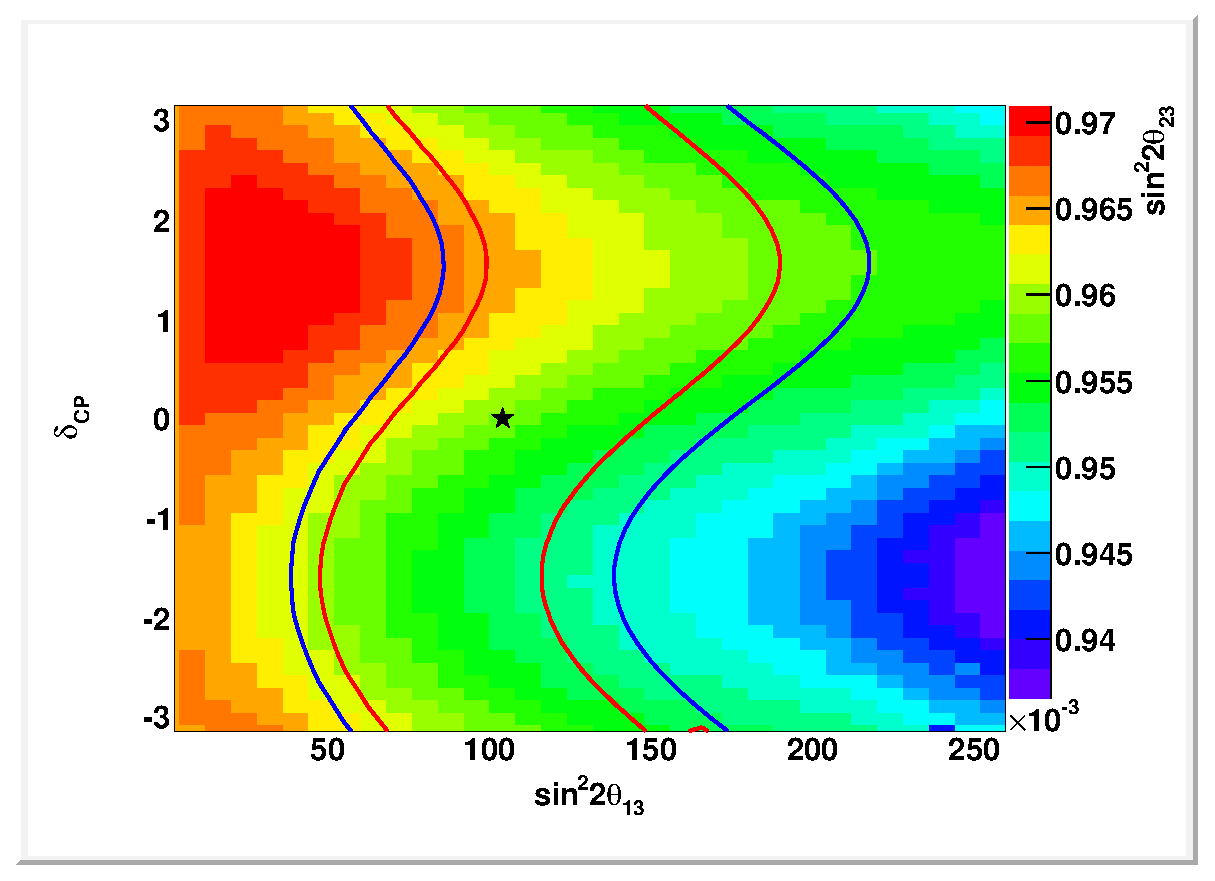
\includegraphics[width=0.5\textwidth]{images/validation/FittedTheta23JointFit.eps}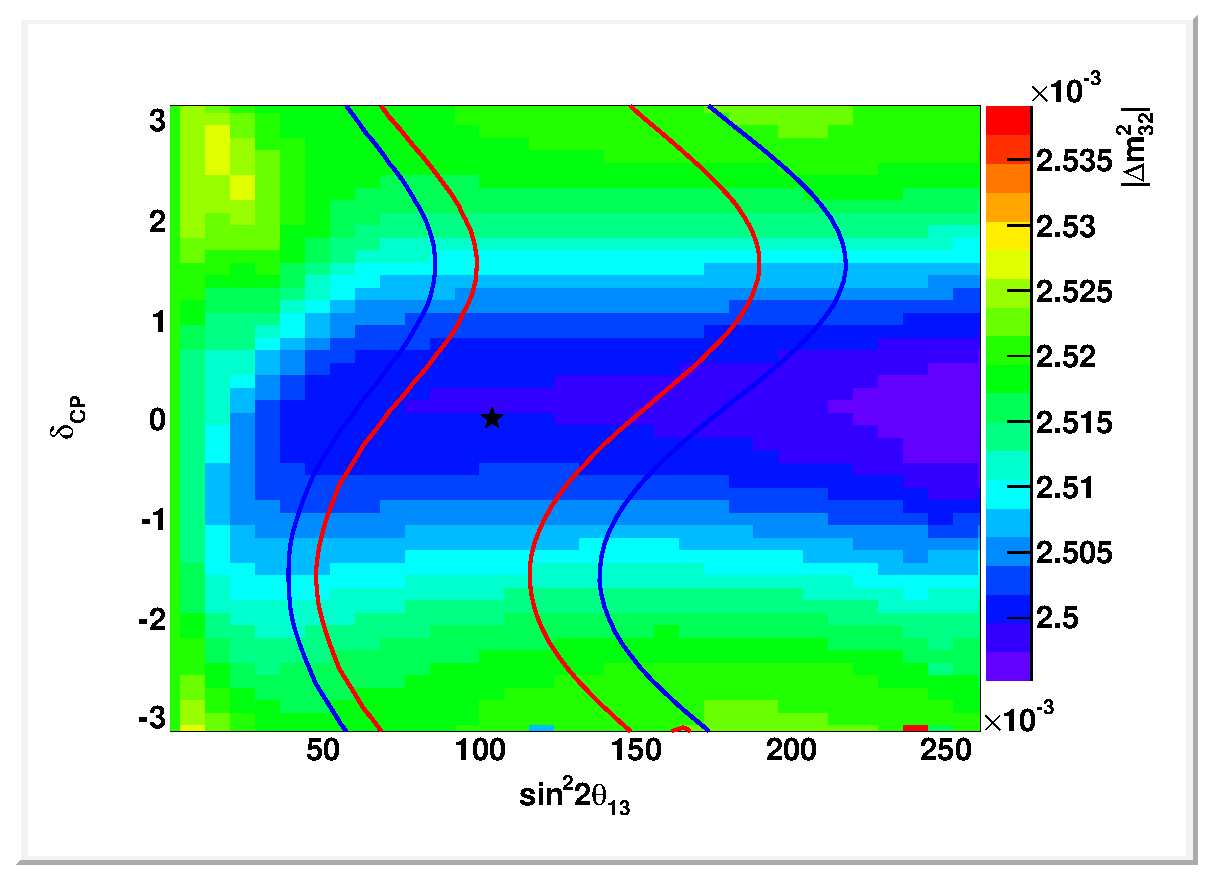
\includegraphics[width=0.5\textwidth]{images/validation/FittedDm23sqJointFit.eps}
\caption{Fitted values of the two marginalised parameters $\sin^{2}2\theta_{23}$ (left) and $\Delta m_{32}^{2}$ (right) for the joint oscillation analysis in the 
$\sin^{2}2\theta_{13}$-$\delta_{CP}$ parameter space for the estimated final POT (7$\times$10$^{21}$). The confidence contours are superimposed for comparison.}
\label{fig:jointappfitted}
\end{center}
\end{figure}


\begin{figure}[htbp]
\begin{center}
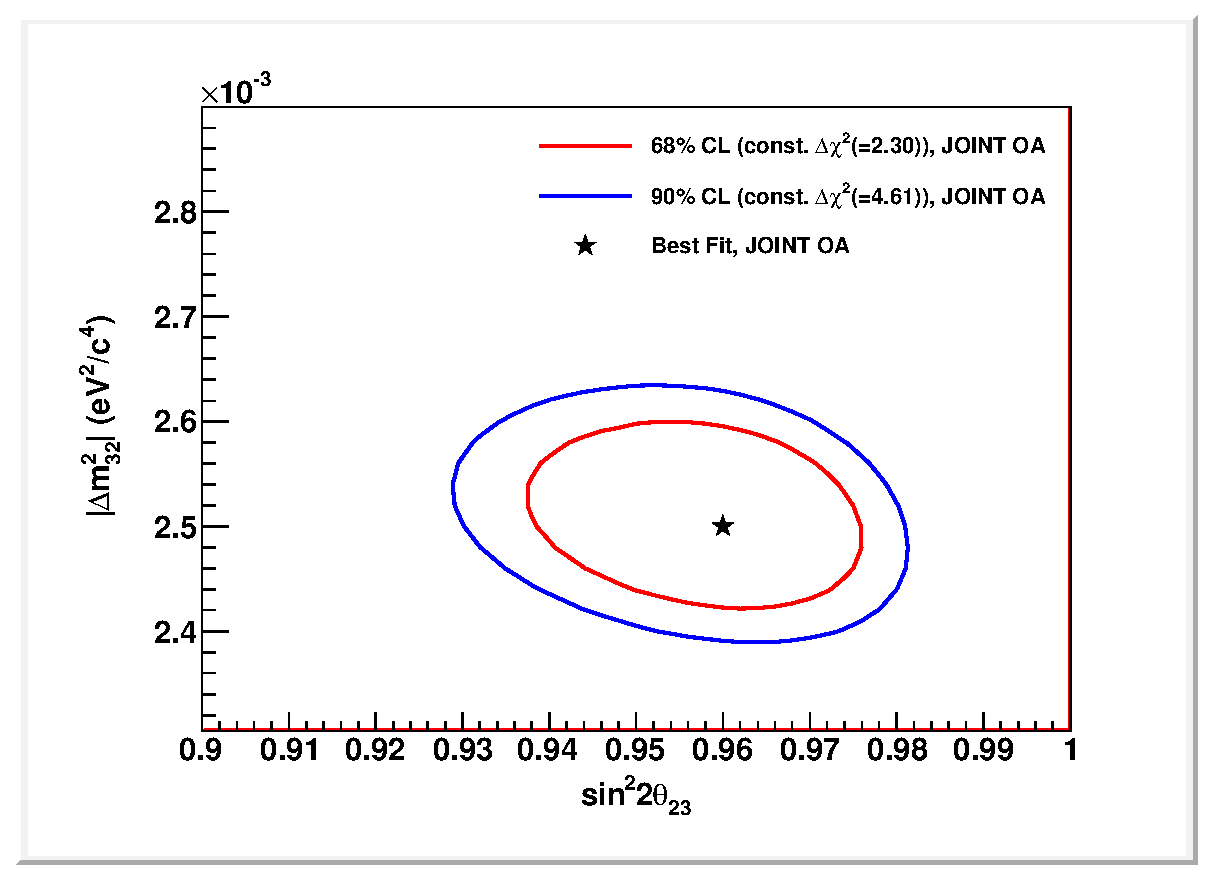
\includegraphics[width=0.7\textwidth]{images/validation/DisappContoursJointOAMock100New.eps}
\caption{2D confidence regions for the joint oscillation analysis in the $\sin^{2}2\theta_{23}$-$\Delta m_{32}^{2}$ parameter space for the estimated final POT (7$\times$10$^{21}$). }
\label{fig:jointdisapp}
\end{center}
\end{figure}

 \begin{figure}[htbp]
\begin{center}
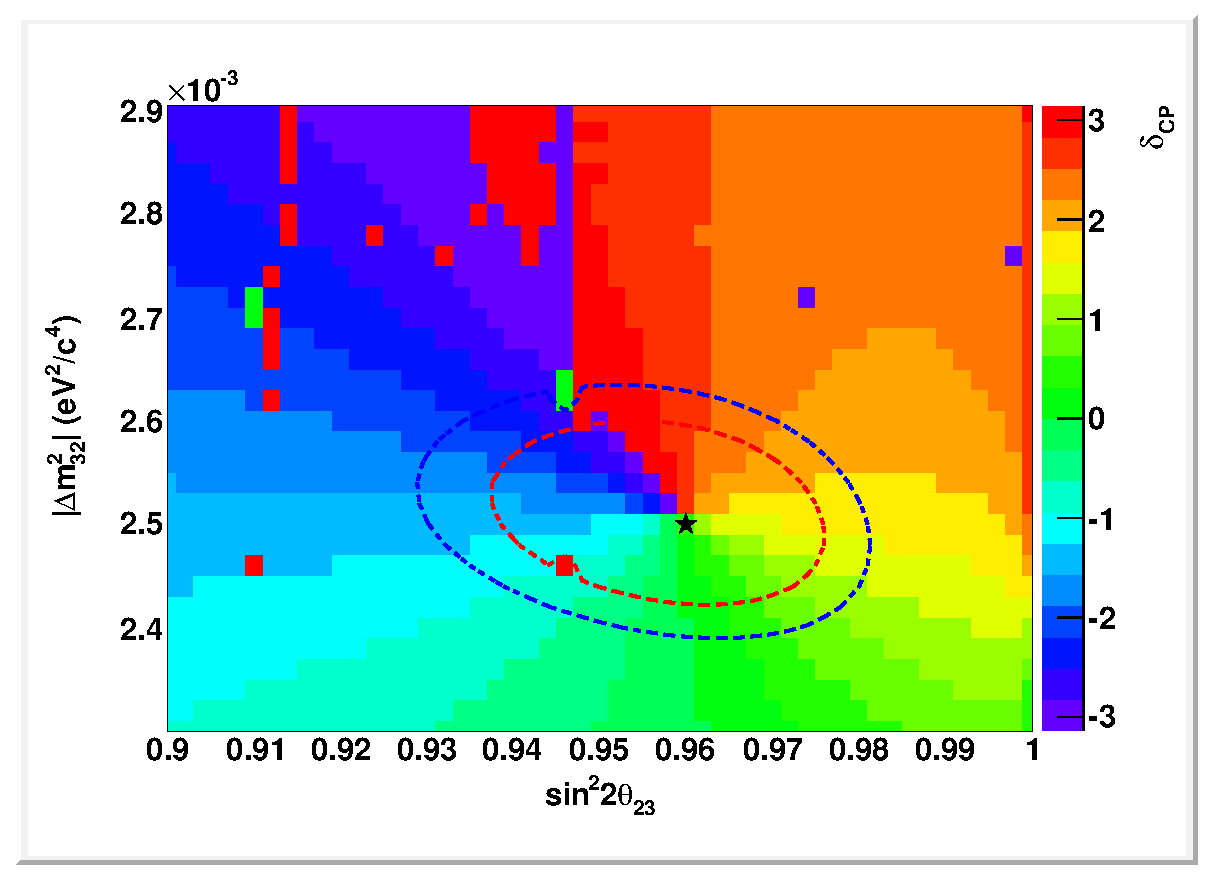
\includegraphics[width=0.5\textwidth]{images/validation/FittedDeltaCPJointFit.eps}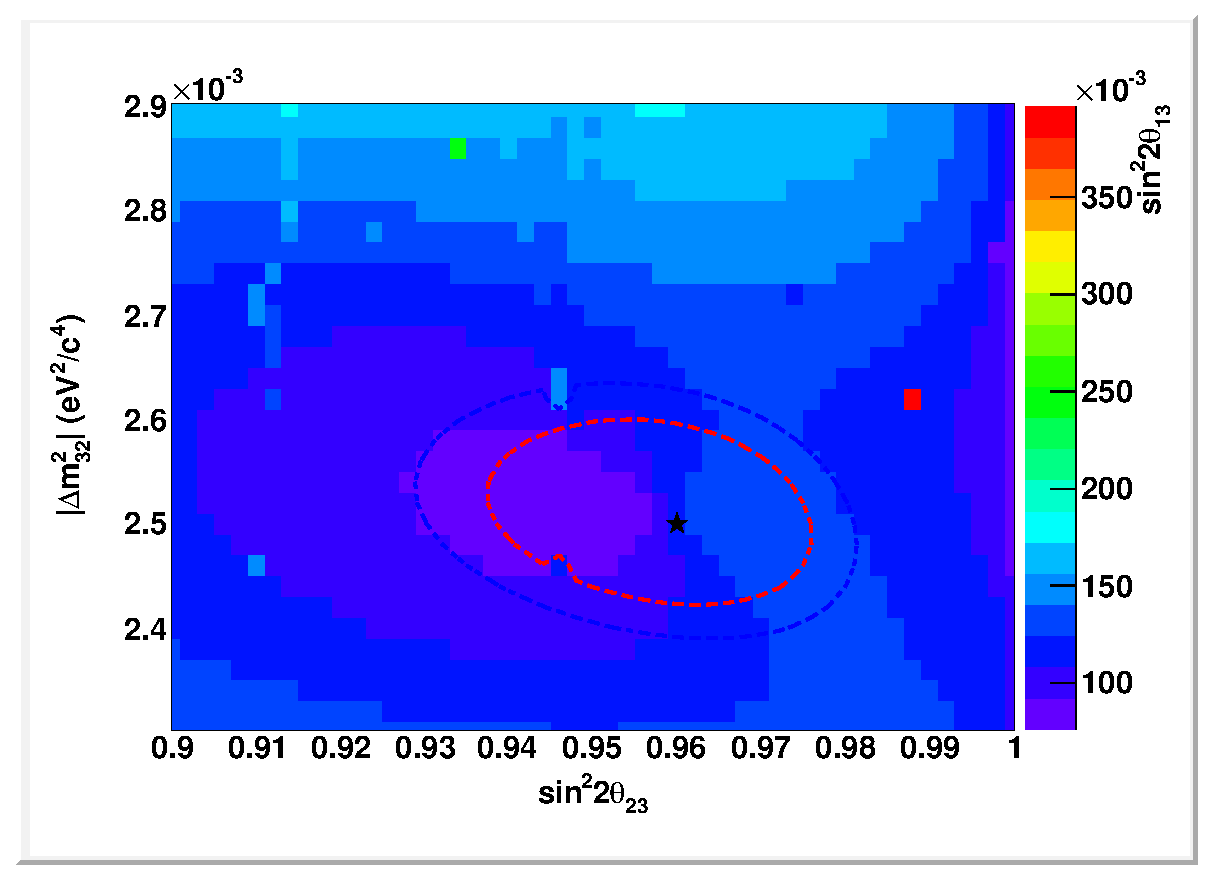
\includegraphics[width=0.5\textwidth]{images/validation/FittedTheta13JointFit.eps}
\caption{Fitted values of the two marginalised parameters $\delta_{CP}$ (left) and $\sin^{2}2\theta_{13}$ (right) for the joint oscillation analysis in the 
$\sin^{2}2\theta_{23}$-$\Delta m_{32}^{2}$ parameter space for the estimated final POT (7$\times$10$^{21}$). The confidence contours are superimposed 
for comparison.}
\label{fig:jointdisappfitted}
\end{center}
\end{figure}

\clearpage


Again the true input values were recovered by the fitter for all oscillation parameters except $\delta_{CP}$, and this is shown in Table \ref{tab:jointOAbestfit}.
In this table, the best-fit values of two parameters are at the centre of the 2D grid rectangle where the best fit was found, while the best-fit values of the other
two marginalised parameters are their fitted values at that point.

\begin{table}[h]
\centering
\begin{tabular}{|c|c|c|c|c|}
\hline
  & $\sin^{2}2\theta_{23}$ & $\Delta m_{32}^{2} (10^{-3} eV^{2}/c^{4})$  & $\sin^{2}2\theta_{13}$ & $\delta_{CP}$ \\
\hline \hline
{\color{blue}{True input values}} & {\color{blue}{0.96}} & {\color{blue}{2.5}} & {\color{blue}{0.12}} & {\color{blue}{0.5}} \\
\hline 
Best-fit point ($\sin^{2}2\theta_{13}$-$\delta_{CP}$ space &  0.958& 2.499& 0.104 &  0\\
 with $\sin^{2}2\theta_{23}$ and $\Delta m_{32}^{2}$ marginalised) &  &  &  &  \\
\hline 
Best-fit point ($\sin^{2}2\theta_{23}$-$\Delta m_{32}^{2}$ space & 0.96 & 2.5 & 0.12003 & 0.501\\
with $\sin^{2}2\theta_{13}$ and $\delta_{CP}$ marginalised) &  &  &  &  \\
\hline
\end{tabular}
\caption{Comparison of the true input oscillation parameters with the best-fit points from the joint oscillation fit. In the second row, the values of 
$\sin^{2}2\theta_{13}$ and $\delta_{CP}$ are the central values of the 2D grid rectangle where the best fit was found, while the values of $\sin^{2}2\theta_{23}$ 
and $\Delta m_{32}^{2}$ are the fitted values at that point. In the third row, the values of $\sin^{2}2\theta_{23}$ and $\Delta m_{32}^{2}$ are the 
central values of the best-fit 2D grid rectangle, and $\sin^{2}2\theta_{13}$ and $\delta_{CP}$ the fitted values at that point.}
\label{tab:jointOAbestfit}
\end{table}
The true input value of $\delta_{CP}$ was 0.5, and its global best-fit value in the $\sin^{2}2\theta_{13}$-$\delta_{CP}$ parameter space was 0; however 
further inspection revealed a second minimum in $\Delta\chi^{2}$ at $\delta_{CP}$ = 0.5 whose value of $\chi^{2}$ was only 1$\times$10$^{-5}$ greater 
than the global minimum. 

Several stand-alone analyses were also performed for comparison with the joint analysis. The stand-alone $\nu_{\mu}$-disappearance analysis used only 
the first and third terms in equation \ref{eq:chisqtot}, while the stand-alone $\nu_{e}$-appearance analysis used only the second and third terms. Also only 
those systematic uncertainties relevant to the single $\mu$-like ring sample were considered in the $\nu_{\mu}$-disappearance analysis, and only those relevant 
to the single e-like ring sample in the $\nu_{e}$-appearance analysis (see table \ref{tab:systematicslist}). However in other respects these stand-alone analyses 
were done in the same way as the joint analysis: systematic parameters were allowed to float in the fit, and the contours were drawn using the 
constant-$\Delta \chi^{2}$ method. 

There are several ways to compare the 2D confidence contours between the joint and stand-alone analyses. For example, a fit in two steps will now be described 
that imitates the stand-alone analyses. In this study, the true input values of the oscillation parameters to the toy MC are identical to those in 
table \ref{tab:jointOAbestfit}. 

\renewcommand{\labelitemi}{$\bullet$} 

\labelitemi{ \textbf{Step I : Stand-alone $\nu_{e}$-appearance analysis fixing $\sin^{2}2\theta_{23}$ to maximal.}}
As mentioned in section \ref{sec:motivation}, a stand-alone $\nu_{e}$-appearance analysis usually assumes that $\sin^{2}2\theta_{23}$ is maximal. But 
small changes in this parameter can have quite large effects on the best fit and the confidence contours: this is shown in figure \ref{fig:appstand}, 
which compares the $\sin^{2}2\theta_{13}$-$\delta_{CP}$ best fit and confidence contours from a fit to a toy experiment fitted assuming $\sin^{2}2\theta_{23}$ = 1.0 
with those from a fit assuming it is 0.96 (the true input value). Clearly there is a bias in both the best fit and the contours when the ``wrong'' value 
of $\sin^{2}2\theta_{23}$ is assumed. This bias can be removed by using the joint analysis, i.e.\ by using all three terms in equation \ref{eq:chisqtot} and 
fitting all four oscillation parameters, and this is shown in figure \ref{fig:appstandjoint}. 

\begin{figure}[htbp]
\begin{center}
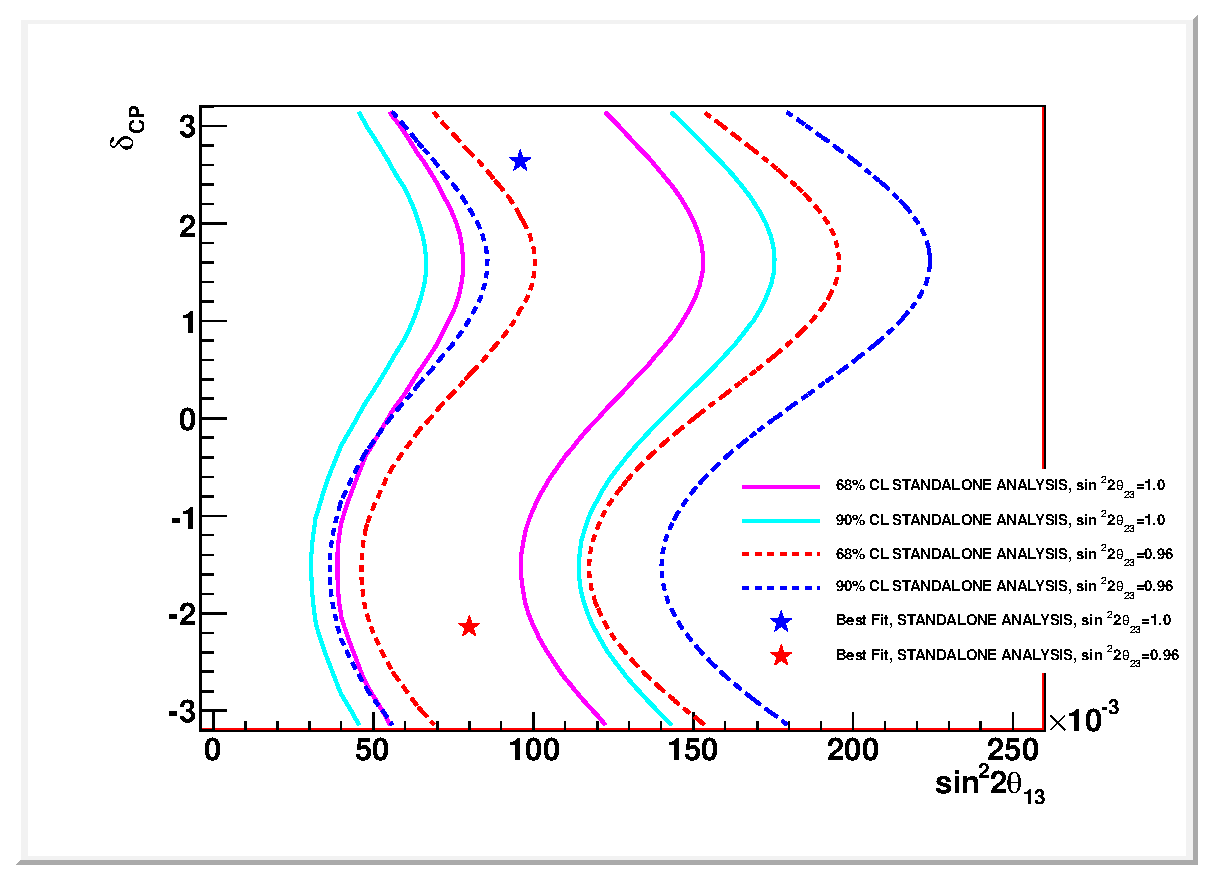
\includegraphics[width=0.7\textwidth]{images/validation/AppContoursMock100FixedVsFixedTrue.eps}
\caption{Comparison of best fit and 2D confidence regions in the $\sin^{2}2\theta_{13}$-$\delta_{CP}$ parameter space for the stand-alone appearance analysis fixing 
$\sin^{2}2\theta_{23}$ to 1.0 (light colors, solid lines) with those fixing $\sin^{2}2\theta_{23}$ to the true input value of 0.96 (dark colors, dashed lines) 
for the estimated final POT (7$\times$10$^{21}$).}
\label{fig:appstand}
\end{center}
\end{figure}

\begin{figure}[htbp]
\begin{center}
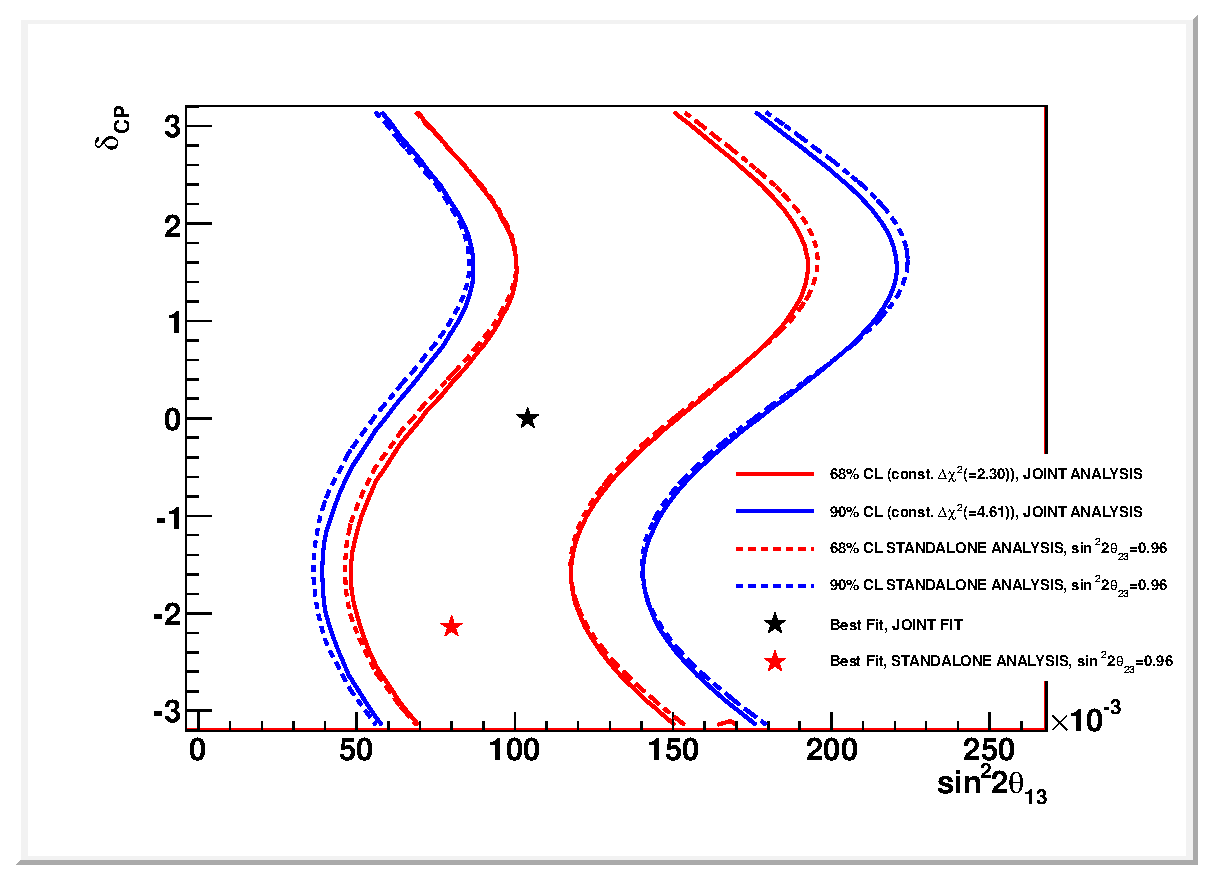
\includegraphics[width=0.7\textwidth]{images/validation/AppContoursJointOAMock100NewVsFixedTrue.eps}
\caption{Comparison of best fit and 2D confidence regions in the $\sin^{2}2\theta_{13}$-$\delta_{CP}$ parameter space for the stand-alone appearance analysis 
fixing $\sin^{2}2\theta_{23}$ to the true input value of 0.96, (dark colors, dashed lines) with those obtained using the joint oscillation analysis (dark colors, 
solid lines) for the estimated final POT (7$\times$10$^{21}$).}
\label{fig:appstandjoint}
\end{center}
\end{figure}

\labelitemi{ \textbf{Step II : Stand-alone $\nu_{\mu}$-disappearance analysis fixing $\sin^{2}2\theta_{13}$ to best-fit value from step I. }}
In this second step, the stand-alone $\nu_{\mu}$-disappearance analysis is done with $\sin^{2}2\theta_{13}$ fixed in the fit to 0.08, its best-fit value from 
step 1, and $\delta_{CP}$ fixed to 0. A comparison is shown in figure \ref{fig:disappstandjoint} of the best fit and confidence contours from the stand-alone 
analysis under these circumstances with those from the joint analysis in which all four oscillation parameters are fitted. Again there is a bias in the best fit 
for the stand-alone analysis, while the confidence contours are rotated compared with those from the joint analysis. 

\begin{figure}[htbp]
\begin{center}
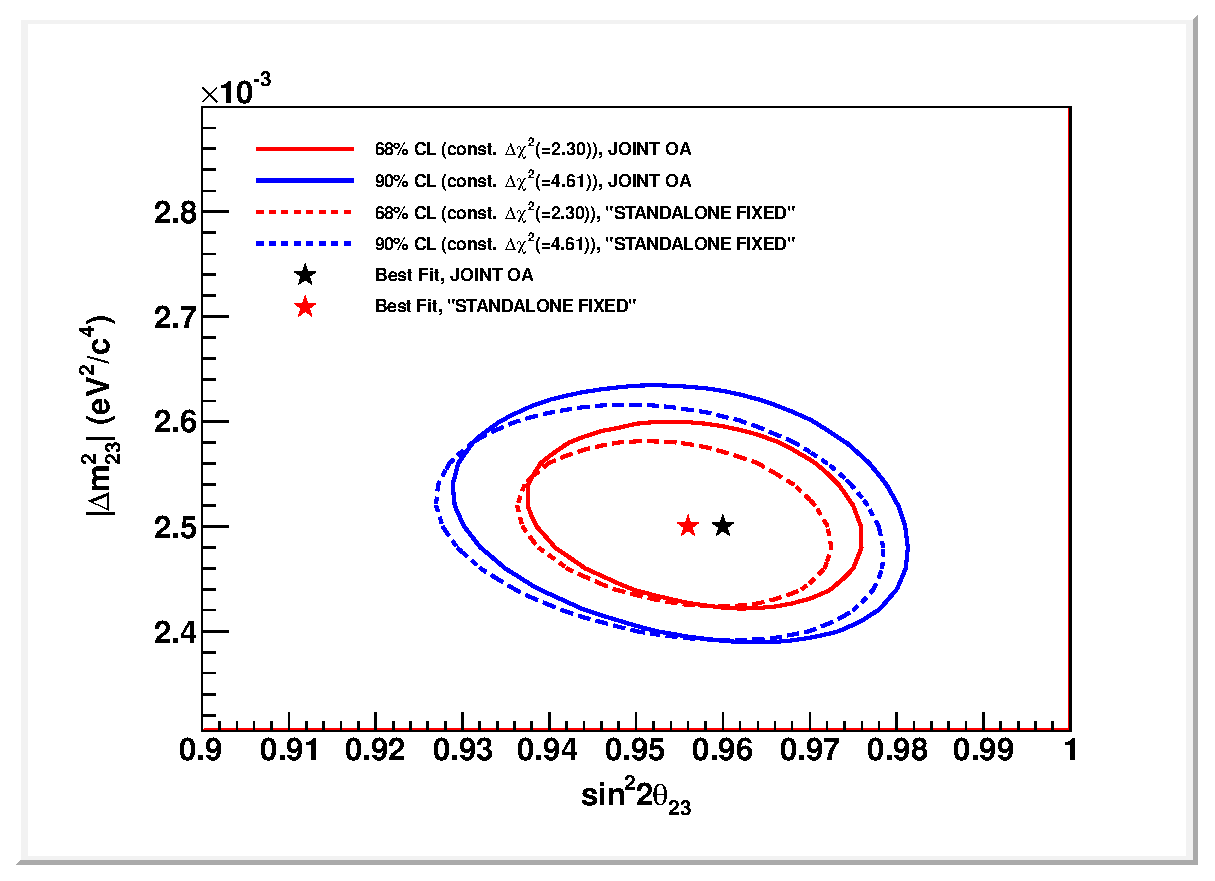
\includegraphics[width=0.7\textwidth]{images/validation/DisappContoursJointOAMock100NewVsFixed.eps}
\caption{Comparison of best fit and 2D confidence regions in the $\sin^{2}2\theta_{23}$-$\Delta m_{32}^{2}$ parameter space for the stand-alone 
$\nu_{\mu}$-disappearance analysis fixing $\sin^{2}2\theta_{13}$ = 0.08 (from fit in figure \ref{fig:appstand}) and $\delta_{CP}$ = 0 (dashed lines) with those 
from the joint analysis (solid lines) for the estimated final POT (7$\times$10$^{21}$).}
\label{fig:disappstandjoint}
\end{center}
\end{figure}

The results in figures \ref{fig:appstandjoint} and \ref{fig:appstandjoint} clearly show the advantages of using the joint oscillation analysis instead of separate 
$\nu_{e}$-appearance and $\nu_{\mu}$-disappearance analyses. 

It might be expected that the confidence regions would be larger in the joint analysis that in the stand-alone analyses since two extra oscillation parameters are 
fitted. However the sizes of the confidence regions are similar, and this is because the joint analysis fits both the one e-like ring and one $\mu$-like ring Super K 
samples, whereas a stand-alone analysis fits only one of them. Thus the joint analysis takes into account the extra information needed to fit the additional parameters. 
A study was made of fitting two extra parameters without adding the necessary information using a stand-alone $\nu_{\mu}$-disappearance analysis; in this analysis, 
$\sin^{2}2\theta_{23}$ and $\Delta m_{32}^{2}$ were fitted while $\sin^{2}2\theta_{13}$ and $\delta_{CP}$ were marginalised using only the one $\mu$-like ring sample. 
The confidence contours were larger than when only two parameters were fitted, and this is shown in figure \ref{fig:disappstandfitjoint}. 

\begin{figure}[htbp]
\begin{center}
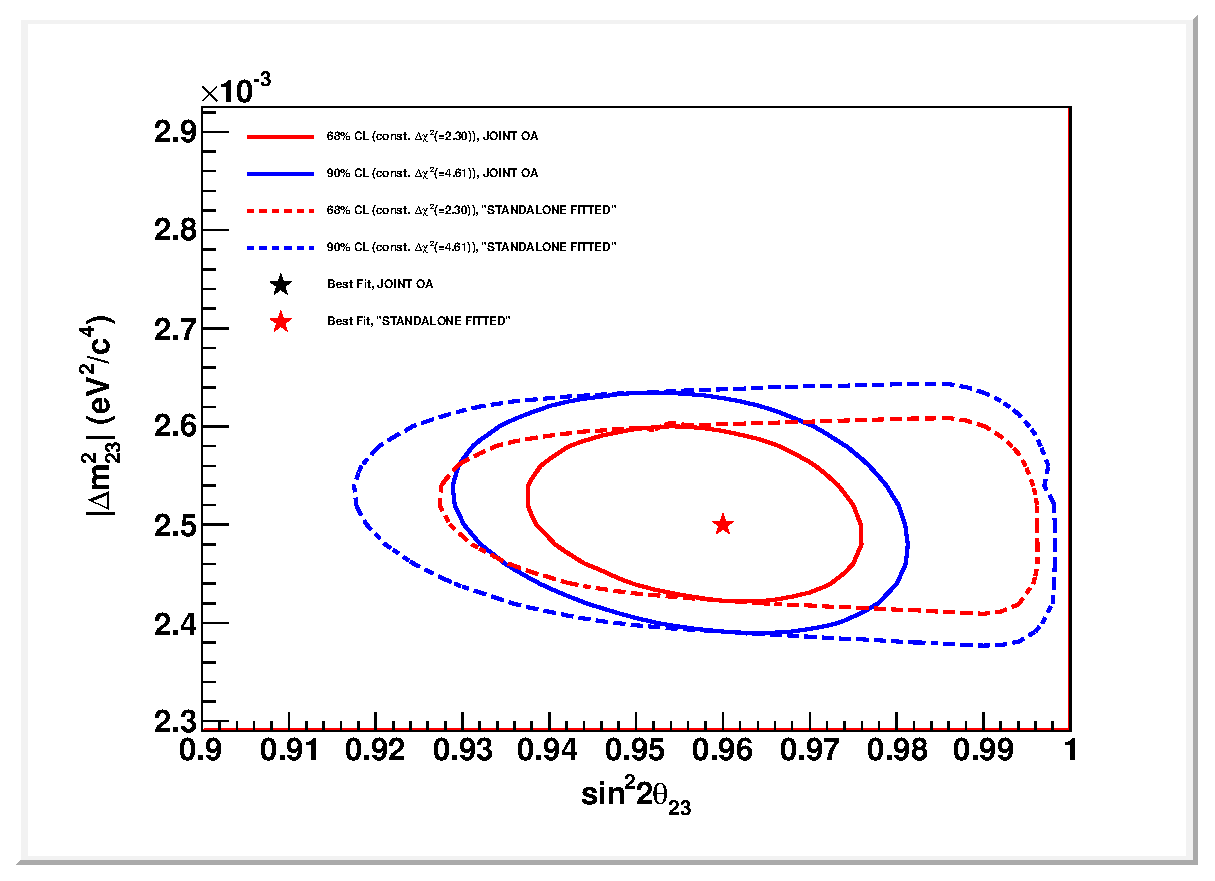
\includegraphics[width=0.7\textwidth]{images/validation/DisappContoursJointOAMock100NewVsFitted.eps}
\caption{Comparison of best fit and 2D confidence regions in the $\sin^{2}2\theta_{23}$-$\Delta m_{32}^{2}$ parameter space for the stand-alone $\nu_{\mu}$-disappearance 
analysis marginalizing $\delta_{CP}$ and $\sin^{2}2\theta_{13}$ (dashed lines) with those obtained using the joint oscillation analysis (solid lines) for the estimated 
final POT (7$\times$10$^{21}$).}
\label{fig:disappstandfitjoint}
\end{center}
\end{figure}
The odd shape of the confidence contours from the stand-alone analysis in figure \ref{fig:disappstandfitjoint} is due to the parameters $\sin^{2}2\theta_{13}$ and 
$\delta_{CP}$ not being fitted correctly when they are marginalised. As shown in figure \ref{fig:disappstandfitted}, the fitted values of these parameters are at 
the upper or lower limits of their allowed ranges. This occurs because the information needed to fit them is not contained in the one $\mu$-like ring SuperK sample.

\begin{figure}[htbp]
\begin{center}
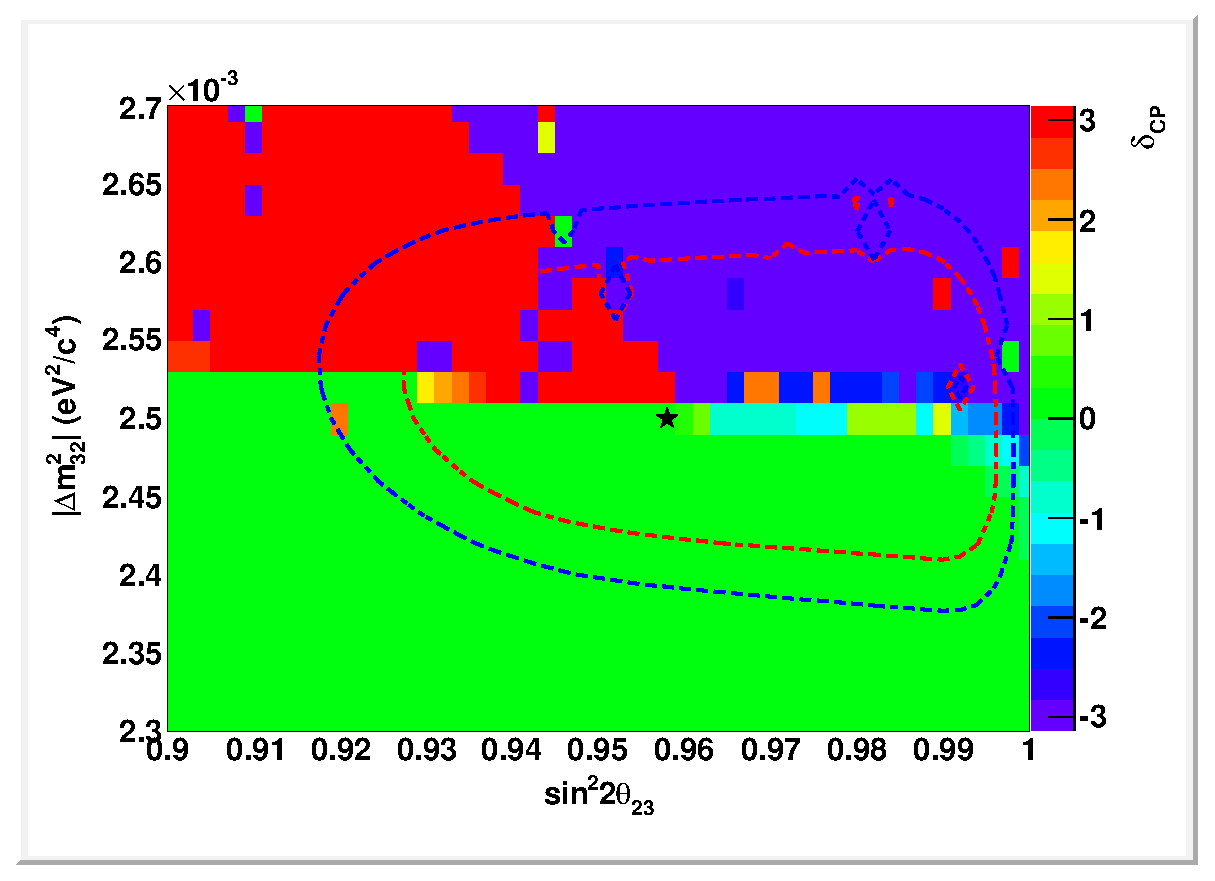
\includegraphics[width=0.5\textwidth]{images/validation/FittedDeltaCPStandFitted.eps}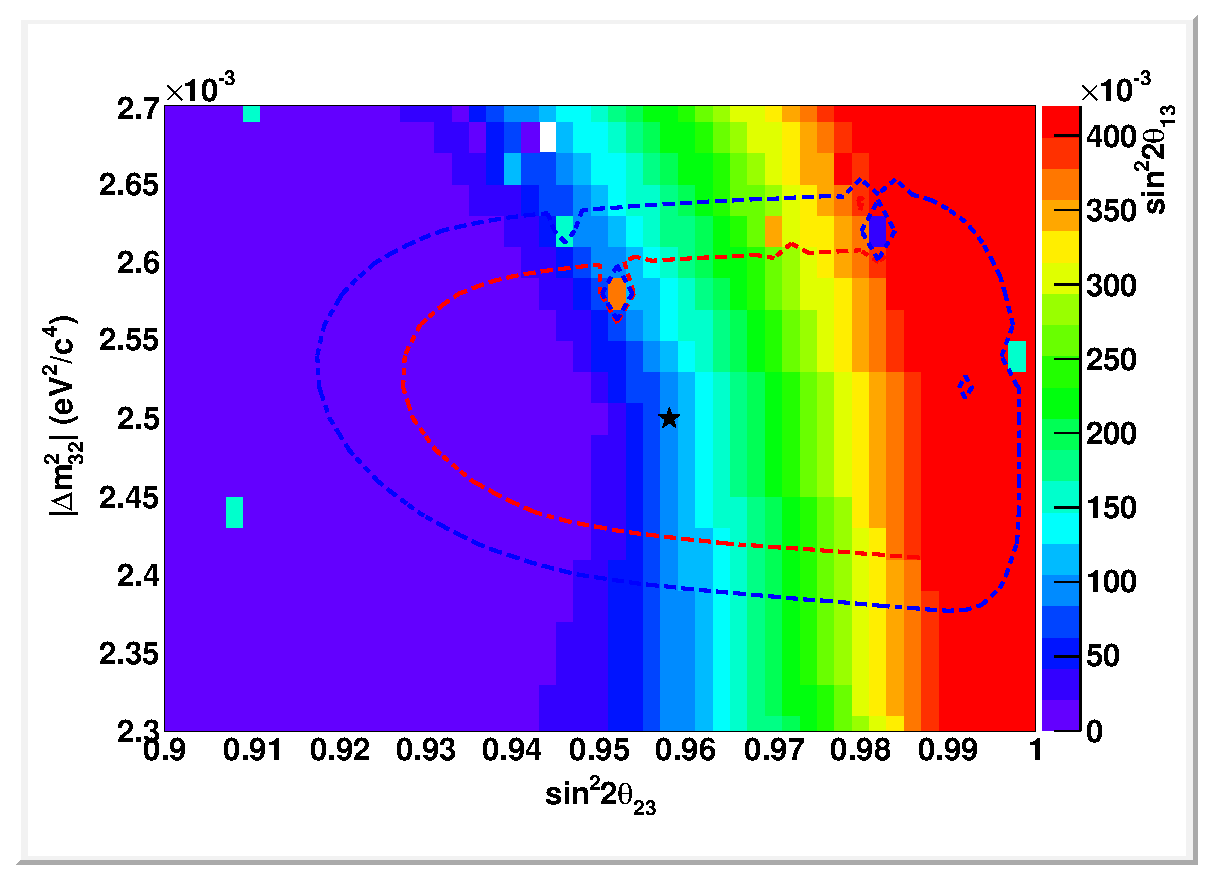
\includegraphics[width=0.5\textwidth]{images/validation/FittedTheta13PStandFitted.eps}
\caption{Fitted values of $\delta_{CP}$ (left) and $\sin^{2}2\theta_{13}$ (right) for the stand-alone $\nu_{\mu}$-disappearance analysis in which they are marginalised 
for the estimated final POT (7$\times$10$^{21}$).}
\label{fig:disappstandfitted}
\end{center}
\end{figure}

